\documentclass[letterpaper,12pt]{article}
\usepackage[usenames,dvipsnames,svgnames,table]{xcolor}
\usepackage{graphicx}
\usepackage{caption}
\usepackage{subcaption}
\usepackage{tabularx}
\usepackage{amsmath,amssymb}
\usepackage{mathrsfs}
\usepackage{setspace}
\usepackage{enumerate}
\usepackage{todonotes}
\usepackage{listings}
\usepackage{paralist}
\usepackage{natbib}
\usepackage{fullpage}
\usepackage[T1]{fontenc}
\usepackage{booktabs}
\usepackage{pgfplotstable}
\usepackage{makecell}
\usepackage{comment}
\usepackage{soul}
\usepackage{bm}
\usepackage{gensymb}
\usepackage{todonotes}
\usepackage{multirow}

\usepackage[colorlinks=true,
            linkcolor=blue,
            urlcolor=blue,
            citecolor=blue,
            final,
            hypertexnames=true]{hyperref}
\newcommand\myworries[1]{\textcolor{red}{#1}}
\newcommand{\abs}[1]{\ensuremath{ \left|#1\right|}}
\newcommand{\norm}[1]{\ensuremath{ \left|\left|#1\right|\right|}}
\newcommand{\orderof}[1]{\ensuremath{ {\cal O}\left(#1\right)}}
\newcommand{\pdv}[2]{\frac{\partial #1}{\partial #2}}
\newcommand{\grad}[1]{\bv{\nabla} {#1}}
\newcommand{\bv}[1]{{\ensuremath{\boldsymbol{#1}}}}
\newcommand{\bt}[1]{{\ensuremath{\boldsymbol{#1}}}}
\newcommand{\Res}{{\ensuremath{\mathcal R}}}
\newcommand{\Unknowns}{{\ensuremath{\bf{U}}}}
\newcommand{\UnknownsR}{{\ensuremath{\bf{U^R}}}}
\newcommand{\unknown}{{\ensuremath{\bv{u}}}}
\newcommand{\primalsol}{{\ensuremath{\bv{\tilde{u}}}}}
\newcommand{\primalsolh}{{\ensuremath{\bv{\tilde{u}^h}}}}
\newcommand{\adjointsol}{{\ensuremath{\bv{\tilde{z}}}}}
\newcommand{\adjointsolh}{{\ensuremath{\bv{\tilde{z}^h}}}}
\newcommand{\adjointsolH}{{\ensuremath{\bv{\tilde{z}^H}}}}
\newcommand{\Testfuncs}{{\ensuremath{\bf{V}}}}
\newcommand{\testfunc}{{\ensuremath{\bv{v}}}}
\newcommand{\intO}{\ensuremath{\int_\Omega}}
\newcommand{\elem}{\ensuremath{E}}
\newcommand{\qoi}{{\ensuremath{q}}}
\newcommand{\qoih}{\ensuremath{q^h}}
\newcommand{\Qoi}{{\ensuremath{Q}}}
\newcommand{\param}{{\ensuremath{\xi}}}
\newcommand{\params}{{\ensuremath{\bv{\param}}}}
\newcommand{\PDF}{\ensuremath{p}}
\newcommand{\Params}{{\ensuremath{\bf{\Xi}}}}
\newcommand{\ParamsR}{{\ensuremath{\bf{\Xi^R}}}}
\newcommand{\Reals}{{\ensuremath{\mathbb{R}}}}
\newcommand{\sa}{\nu_{\mathrm{sa}}}
\newcommand{\pp}[2]{\frac{\partial #1}{\partial #2}}

%
\newcommand{\uveci}{{\bm{\hat{\textnormal{\bfseries\i}}}}}
\newcommand{\uvecj}{{\bm{\hat{\textnormal{\bfseries\j}}}}}
\newcommand{\uveck}{{\bm{\hat{\textnormal{\bfseries\k}}}}}


\author{Nicholas Malaya}

\begin{document}

%%%%%%%%%%%%%%%%%%%%%%%%%%%%%%%%%%%%%%%%%
% University Assignment Title Page 
% LaTeX Template
% Version 1.0 (27/12/12)
%
% This template has been downloaded from:
% http://www.LaTeXTemplates.com
%
% Original author:
% WikiBooks (http://en.wikibooks.org/wiki/LaTeX/Title_Creation)
%
% License:
% CC BY-NC-SA 3.0 (http://creativecommons.org/licenses/by-nc-sa/3.0/)
% 
% Instructions for using this template:
% This title page is capable of being compiled as is. This is not useful for 
% including it in another document. To do this, you have two options: 
%
% 1) Copy/paste everything between \begin{document} and \end{document} 
% starting at \begin{titlepage} and paste this into another LaTeX file where you 
% want your title page.
% OR
% 2) Remove everything outside the \begin{titlepage} and \end{titlepage} and 
% move this file to the same directory as the LaTeX file you wish to add it to. 
% Then add \input{./title_page_1.tex} to your LaTeX file where you want your
% title page.
%
%%%%%%%%%%%%%%%%%%%%%%%%%%%%%%%%%%%%%%%%%

%----------------------------------------------------------------------------------------
%	PACKAGES AND OTHER DOCUMENT CONFIGURATIONS
%----------------------------------------------------------------------------------------

%\documentclass[12pt]{article}

%\begin{document}

\begin{titlepage}

\newcommand{\HRule}{\rule{\linewidth}{0.5mm}} % Defines a new command for the horizontal lines, change thickness here

\center % Center everything on the page
 
%----------------------------------------------------------------------------------------
%	HEADING SECTIONS
%----------------------------------------------------------------------------------------

\textsc{\LARGE Doctoral Dissertation Proposal}\\[1.5cm] % Name of your university/college

%----------------------------------------------------------------------------------------
%	TITLE SECTION
%----------------------------------------------------------------------------------------

\HRule \\[0.4cm]
{ \Large \bfseries Numerical Simulation of Synthetic, Buoyancy-Induced Columnar Vortices}\\[0.4cm] % Title of your document
\HRule \\[1.5cm]
\textsc{\Large Nicholas Malaya}\\[0.5cm] % Major heading such as course name
\textsc{\large Department of Mechanical Engineering}\\[2.5cm] % Minor heading such as course title
 
%----------------------------------------------------------------------------------------
%	AUTHOR SECTION
%----------------------------------------------------------------------------------------

\begin{minipage}{0.4\textwidth}
\begin{flushleft} \large
{}%{\Huge Nicholas Malaya} \\
%{\normalsize Department of Mechanical Engineering} 
\end{flushleft}
\end{minipage}
~
\begin{minipage}{0.4\textwidth}
\begin{flushright} \large
\emph{Committee:} \\
 \vspace{5mm}
{\Large Dr. Robert D. Moser} \\
{\normalsize \textsl{Advisor}} \\
{\normalsize Department of Mechanical Engineering and Institute for Computational Engineering and Science} \\
 \vspace{5mm}
{\Large Dr. David Bogard} \\
{\normalsize Department of Mechanical Engineering} \\
 \vspace{5mm}
{\Large Dr. Todd A. Oliver} \\
{\normalsize Institute for Computational Engineering and Science} \\
 \vspace{5mm}
{\Large Dr. Venkat Raman} \\
{\normalsize Department of Aerospace Engineering and Engineering Mechanics} \\
\end{flushright}
\end{minipage}\\[4cm]

%----------------------------------------------------------------------------------------
%	DATE SECTION
%----------------------------------------------------------------------------------------

%{\large \today}\\[3cm] % Date, change the \today to a set date if you want to be precise

%----------------------------------------------------------------------------------------
%	LOGO SECTION
%----------------------------------------------------------------------------------------

%\includegraphics{Logo}\\[1cm] % Include a department/university logo - this will require the graphicx package
 
%----------------------------------------------------------------------------------------

\vfill % Fill the rest of the page with whitespace

\end{titlepage}
%\end{document}


\newpage
\begin{abstract}
\doublespacing

turbulence

\end{abstract}


\newpage
\tableofcontents
\newpage
%\singlespacing
\onehalfspacing
%\doublespacing
\section{Introduction / Executive Summary}

Renewable energy is critical to our environmental, economic, and
national security. Demand for energy is on the rise, as is our national
reliance on fossil fuel-based power plants for the bulk of our
electricity generation. There is a critical need for safe, clean, and
cost-effective alternatives to coal, such as wind, solar, hydroelectric,
and geothermal power\cite{arpa-e}. These technologies would reduce carbon dioxide
emissions and help position the U.S. as a leader in the global renewable
energy industry. 
%
% proposal
%
This proposal details a research plan perform a numerical investigation
for the design and optimization of a novel device for renewable, clean
energy generation. 

Much of the solar energy incident on the Earth's surface is absorbed
into the ground, which in turn heats the air layer above the surface.
This buoyant air layer contains considerable gravitational potential
energy. 
With nearly one-third of global land mass covered by deserts, there are huge
untapped regions for capturing solar heat (about 200 W/$\text{m}^2$ averaged over
a 24-hour day, and up to 1000 W/$\text{m}^2$ peak).  The available power is
competitive in magnitude with worldwide power generation from fossil
sources. If successful, this could result in a low-cost, scalable
approach to electrical power generation that could create a new class of
renewable energy ideally suited for arid low-wind regions. 

How then, is one to efficiently extract this gravitational potential
energy and convert it into useable work? We turn to Nature to provide a 
guide, with the observation that objects already
exist that provide precisely this mechanism. Namely, the phenomena is
that of a naturally 
%
% are we certain this is baroclinic? montegomery might argue it is not.
% update: I think montgomery is wrong here, or at best nitty.  
% BAROCLINIC: essentially just that temp fronts exist
%
occurring ``dust devil'' with baroclinic generation of vorticity in a
vertically stratified, ground-heated air layer producing a coherent
columnar vortex. These ``dust-devil''s are naturally appearing in
regions as diverse as Arizona, to over water, to Mars\cite{mars}. They
are observed to occur over a wide range of length scales (between )with
large variations in 
velocities ()\cite{sinclair}. 

Thus, the basic idea behind this engineering approach is to convert the 
potential energy in this buoyant air layer to kinetic energy in an
anchored vortex, and to use that kinetic energy to drive a
vertical-axis turbine coupled with an electric generator in order to
produce electrical power. 
The Solar-Driven Vortex (SoV) phenomena has already been demonstrated in
an experimental setup by our partners at Georgia Tech. The simulation
effort intends to utilize Computational Fluid Dynamics (CFD) to simulate
this SoV. 
%
% TODO: add table of 'state of the art' or novel work performed
%


This proposal outlines a body of research to be performed to build
confidence in the simulation capability, optimize the apparatus, and 
probe the underlying physical dynamics of the system. 
The proposal is organized as follows. In section \ref{sec:physics}, we
begin with a discussion of the physical domain of interest. We then
review the presently understood dynamics of Dust-devils and similar
columnar vorticies. We then utilize this knowledge in section
\ref{sec:model}, in order to motivate a mathematical formulation of the
system of interest. In section \ref{sec:software}, we discuss the 
algorithms and software implementation in order to explicitly solve the
equations of interest and arrive at numerical solutions of our
phenomena. Section \ref{sec:validation} discusses the validation of
these results against existing experimental data and high fidelity
simulations.  Section \ref{sec:results} details the preliminary
predictions of system performance in the field, as well as the
present results of optimization of the apparatus. Finally, section
\ref{sec:future_work} contains a list of remaining tasks necessary to
fufill the goals of this research project. 


%details a short validation
%study performed by comparing between the available experimental
%measurements and the simulations results. 


%In order for these simulations to be generally useful, they must first
%be validated against existing experimental data and high fidelity
%simulations. These models will then explore regimes and scales where no
%experimental measurements presently exist. 
%Characterizing the
%uncertainty of predictions resulting from extrapolation is a critical
%component in enabling reliable assessments of field performance of the
%SoV, as it will guide the commercialization strategy of the product. 


\newpage
\section{Physics of Dust-Devils}
\label{sec:physics}

%% \begin{itemize}
%% \item \st{phenomenological description}
%% \item \st{regions/frequency of occurance}
%% \item \st{review of sinclair, kanak and renno and other pertinent literature}
%% \item \st{known physics of dust devils and other cyclonic structures}
%% \item \st{dust-devil/tornado/hurricane genesis}
%% \item \st{scaling discussion as estimate of energy}
%% \item \st{dust-Devil Generation Concept}
%% \item \st{motivation of computational modeling{
%% \item draw regions
%% %\item eyewall
%% \end{itemize}

In order to motivate how best to \textit{engineer} a synthetic
dust-devil, we first address what is known about the naturally occuring
phenomena. We therefore begin this section with a qualitative discussion
of dust-devils, followed by a review of the known physics and pertinent 
literature review. We then briefly outline how we intend to leverage
these physical processess as a method of usable energy generation. 


\subsection{Phenomenological Character of Dust-Devils}

%\begin{itemize}
%\item chart from sinclair of frequency (they are driven by delta t)
%\item turning direction independent
%\item characteristic velocities and sizes
  %\item genesis diagram (thermal plume) -- mention ambient angular vorticity
%\item structure diagram and description
%\end{itemize}

No rigorous defintion of a Dust devil exists. This cannot be attributed
to the rarity of the processes. Rather, the phenomena of dust devils are
remarkably ubiquitous. These whirlwinds have been
observed across a wide variety of terrains, climates and even on several
other planets\cite{Sinclair1969,Bluestein2004,JGR:JGR13978,JGRE:JGRE1660}. 
While it is difficult to pin down a precise definition, several features 
are characteristic of a dust devil. They are regions of
intense vorticity and rotation, coupled with strong upward motions. 
They are a self-sustaining vortex that maintains a funnel-like
chimney driven by hot air moving both upward and circularly. 
While they typically exist for only a few minutes, some have 
been observed to exist for significantly longer. While the velocities are 
typically several meters per second, 
%
% solen from: http://glossary.ametsoc.org/wiki/Fujita_scale
%
dust devils occasionally are strong enough to cause damage and injury,
with some reaching F1 on the Fujita Tornado intensity scale, with velocities 
between 33 and 49 $m/s$.
%
% F1 (moderate damage): 33-49 m s-1
%
% ``F1 - Surface of roofs peeled off; mobile homes pushed off foundations
% or overturned; moving autos pushed off road. ``
Diameters range from about one meter to greater than thirty.  Their
average height is about thirty meters, but a few have been observed 
as high as 1 km or more. There appears to be no preferred direction, and
they are observed to rotate anticyclonically as well as
cyclonically. Although the vertical velocity 
is predominantly upward, the flow along the a central axis of large dust devils
may be downward. 
%
% cite martian dust devils
%
%Moreover, actual dust devils have been photographed from orbit, with
%some of them as large as 1 to 2 kilometers across at their base and 10
%km tall. 
Similarly visibly structured phenomena have been spotted over water, in
intense forest fires, or even in cold or freezing environments. 
%
% good place to ref jacobson2005fundamentals
%
This is to say nothing of other similar cyclonic phenomena, such as
tornados and hurricanes. 

While the phenomena is pervasive, we can state that certain 
environmental conditions do impact the frequency of formation
of dust devils. Sinclair\cite{Sinclair1969} provides perhaps the most 
systematic investigation characterizing favorable conditions for formation. 

From these results we can conclude that dust devils are most likely 
to form at solar noon, the time of the greatest incident radiation 
on the ground. Furthermore, they are more likely to form in locations 
with a higher surface temperature. 
Moderate to high wind speeds (2-5 m/s) encourage dust 
devil genesis, but greater velocities (11 m/s) appear to impede formation. 
They are more likely to be observed in relatively flat locations, 
such as deserts. 

Actual measurements made inside a dust devil are limited. From what data
is available, the dust devil can be broken into two regions: a low surface 
layer and a higher invisid region. The low surface region is the 
principle location of radial inflow. 
It is at the top of this region that the flow 
reaches its peak velocity, with that peak dropping with increasing height. 
The strong radial and azimuthal velocities are drawn into a low pressure core 
where they gain vertical velocity and are lifted up. Earlier experimental and 
computational results have both observed a cooler downdraft in the very center 
of the dust devil. It is not clear what generates the azimuthal velocities. It is 
possible that ambient vorticity from objects is drawn into the vortex from far 
field, and which intensifies greatly owing to a $1/r^2$ dependence.

The higher region is characterized by a largely invisid potential flow region 
that characterized by warm air rising and circling around a cool, 
low pressure core. This region is typically many times larger in height than the
surface layer. While this region also has radial inflow, but it is 
significantly weaker than the lower region. Previous studies have found that
this region is relatively well described by a Rankine vortex model\cite{}. 
Both of these regions are sketched out as a simple 
cartoon in figure \ref{fig:cartoon}. 

  \begin{figure}[!htb]
    \begin{center}
     \includegraphics[width = 12 cm]{figs/ground}
     \caption{Cartoon of the structure of a dust devil.}
     \label{fig:cartoon}
    \end{center}
  \end{figure}


\subsection{Estimate of Energy Scaling}

Here we provide a rough estimate of the energy
available to a Dust devil. There are two objectives behind this
analysis. The first is to provide justification for the concept of
extracting energy from these phenomena, with the reasoning that should
sufficient energy be available, then attemping to extract it might be
worthwhile. The second objective is to provide a simple analysis that
can serve as a measure of the efficiency of the generation process,
e.g. ``What fraction of the available energy are we extracting?''.  

At present, we consider only the energy flowing into the entrainment
region due to the ambient conditions, in particular, the incoming wind
and heat through the front hemisphere of a cylindrical region. We
consider a medium-sized (3m radius) dust devil with an incoming
freestream velocity of 5 m/s. The surface temperature is 343 Kelvin,
with a specified inflow boundary layer bridging the ground temperature
to the ambient air conditions of 313 Kelvin. 
% cite this?
These numbers were chosen
based on information provided by the Georgia Tech field team in Arizona
during the summer of 2014.  

There are two forms of energy to consider: kinetic and enthalpy. We
begin by considering the kinetic energy flux through the front of the
apparatus. From the first law of thermodynamics we can express the
kinetic energy flux as a surface integral over the upstream face of the device, 
\begin{equation*}
\text{KE} = \int_{CS} \frac{\vec V^2}{2} \rho \vec V \cdot \hat n dA.
\end{equation*}
%
% could cite fluid dynamics book here
% pg. 239
%
We assume our freestream velocity has no components in y and z.
We assume that the variation in z for the streamwise velocity is only on
account of the thin boundary layer near the ground. We functionally
approximate this behavior using the common 7th power function for a
turbulent boundary layer,  
\begin{equation*}
  u(z) = U \text{ min }\left(\left(\frac{z}{\delta}\right)^7,1\right)
\end{equation*}
where U is the constant freestream velocity and $\delta$ the assumed
boundary layer thickness. Our integral can be solved to show, 
\begin{align*}
\text{KE} & = -R \rho U^3 \left[ z_{\text{max}} - \frac{10}{11}\delta.
\right]
\end{align*}

%%  & = \frac{1}{2} R \rho u^3 z_\text{max}
%%  \int^{\frac{3\pi}{2}}_{\frac{\pi}{2}} \text{cos}\theta d\theta \\
%%  & = -R \rho u^3 z_\text{max}. 
%% \end{align*}

The negative sign here indicates that the kinetic energy is flowing into
the surface, in opposition to the outward facing unit normal, $\hat
n$. Characteristic values for this analysis are, $u = 5$ m/s, $\rho =
1.225$ Kg/$m^3$, $R = 3$ m, and $z_{\text{max}} = 2.5$ m. The boundary
layer thickness is $\approx 10$ cm. This provides
an estimate of 1144.26 Watts as the incoming kinetic energy flux. Or,
approximately 1.14 kW.  

We estimate the gravitational potential
energy flux by integrating the boussinesq term by the height of the vanes, 
\begin{align*}
  \text{Potential Energy Flux} & = \int_{-h}^0 u(z) \Delta \rho g z dz. \\
  & = \int_{-h}^0 u(z) \rho' g z^2 dz. 
\end{align*}
Where the substitution, $\Delta \rho = \rho' z$ was made. At 
this point we again separate the integral into two components, 
for the boundary layer and the constant freestream velocity region. 
\begin{align*}
  & = \rho' g \left[ \int_{-\delta}^{0} U \left( \frac{z}{\delta} \right)^7 z^2 dz 
      + \int_{-h}^{-\delta} U z^2 dz \right] \\
  & = -\rho' g U \left[ \frac{h^3}{3} - \frac{7}{30} \delta^3 \right].
\end{align*}
Furthermore, we
note that $\rho' = -\beta \rho_0 \Delta T$, resulting in, 
%
% cite monin-yaglom page 59
%
\begin{equation}
 \text{Power } = U \beta \rho_0 \Delta T g \left[ \frac{h^3}{3} -
					    \frac{7}{30} \delta^3
					   \right]. 
\end{equation}

Using $\rho_0 = 1.225$ Kg/$m^3$, $T_{\text{ref}}=313$m Kelvin, $\beta_T = 0.003194$
(This is just 1/$T_{\text{ref}}$), $g=9.81$ m/$s^2$, and a freesteam
velocity of five meters per second results in an
estimate of 30 Watts for the gravitational potential energy. 

This interesting result implies that the majority of the available
energy is attributable to kinetic energy, not the gravitational
energy. This is consistent with the results of Renno\cite{}, who demonstrated
that the available thermal energy present was not sufficient to account
for the velocities measured in dust devils. However, while the
gravitational potential energy is a small fraction of the energy
available, that does not imply it is without significant impact. The
extend to which the thermal energy acts as an assisting mechanism for 
``lifting-up'' the flow is unclear, but given the observed increase in dust
devil formation during peak thermal gradients, it is certainly expected
to play an important role. 

\subsection{Dust Devil Generation Concept}

The preceeding discussion has provided justification for the idea of
using dust devils as a method of extracting ambient kinetic and
gravitational potential energy from the environment. This  
subsection now provides a brief discussion of how the physics of 
dust devils informs the generation of a synthetic variety. 

In contrast to the naturally occuring dust devils
our synthetic solar driven vortex, (SoV) design makes use of
control surfaces to dictate the
angle of incoming flow, and in doing so explicitly converts a portion of
the incoming radial flow in azimuthal velocity. These turning vanes also
serve as an anchor for the synthetic vortex, locking it into a small
region.  
  \begin{figure}[!htb]
    \begin{center}
     \includegraphics[width = 8 cm]{figs/ground_vanes}
     \caption{Image of a possible two tier turning vane 
       configuration for generating synthetic dust devils.}
     \label{fig:cartoon}
    \end{center}
  \end{figure}

Our principle objective is to use a synthetic dust devil to produce 
useable work. In order to extract this energy, a turbine is placed 
at the top of the vanes, where the blades are driven by the dust devil's 
azimuthal and vertical velocities. 

While the turning vanes and turbine  
paradigm represents a reasonable starting point for design, the
parameter space of possible system configurations is large. It is
unclear how to engineer an effective SoV system. Important design
consideration include: 
\begin{itemize}
  \item How should the turning vanes be configured?
  \item How does the energy produced scale with system diameter?
  \item Could additional surfaces, such as a cone, capable of further 
    increasing energy output?
\end{itemize}

Questions such as these provide the principle impetus of using
computational fluid dynamics (CFD) in order to inform system design. The
parameter space of concievable system designs is far larger than can be
probed experimentally, and even if such a campaign were to be embarked
upon, it would be at significantly greater temporal and monitary
cost. The subseqent chapter will provide the mathematical basis by which
we model the system, so that we can then begin to discuss how we might
optimize it.  




\newpage
\section{Model}

This section uses our blurb from the viscosity document
includes raleigh 
we know the physical regime

then it discusses equations
then it discusses the viscosity model



\subsection{Estimate of the Available Ambient Energy}



\newpage
\section{Computational Methods and Software}
\label{sec:software}

% \begin{itemize}
%  \item \st{discretized equations, finite elements, stabilized}
%  \item penalty formulation, also consider discussing sep model
%  \item \st{software (GRINS+Libmesh)}
%  \item \st{verification of software}
%  \item \st{tool-chain, simulation machine and hardware}
%  \item \st{simulation geometry and boundary conditions for wind/thermal-only}
% \end{itemize}

\subsection{Discretization Scheme}

To solve the Navier-Stokes equations on a computer, a
Galerkin finite element method (FEM) is used, with linear basis
functions for both the velocity and pressure. This scheme circumvents
the Babuska-Brezzi conditions\cite{bb-cond} and 
uses equal-order elements for velocity and 
pressure,  by introducing a stabilization term as first described by
Hughes\cite{Hughes198685} and extended to natural convection as in
Becker and Braack\cite{Becker2002428}.  

The system of ODEs are discretized in time using a theta-method. 
Newton iterations are used to for solve the resulting nonlinear problem. 
The unsteady solver used is typically backward Euler for the
corresponding stability regardless of timestep size. 

\subsection{Penalty Method Implementation}

In the previous section it was noted that a penalty method is used to
represent impermiable surfaces such as the wind block cone. Babuska's
penalty treatment of constraints\cite{1973fempen,ZAMM:ZAMM19880680925}
is used. This was selected because it is easily imposed in the FEM
context, and the method has been explored in detail in the literature. 

In this approach, a penalty for violating the constraint is included in
a variation formulation. As an example, consider Laplace's equation on a
domain $\Omega$ with boundary $\partial\Omega$, 
\begin{equation}
 \nabla^2 u = 0. 
\end{equation}
Dirichlet boundary conditions are introduced into the weak form
\begin{equation}
 u|_{\partial \Omega} = g
\end{equation}
which becomes 
\begin{equation}
\int_{\Omega}  - \nabla u \cdot \nabla v dx - \frac{1}{\epsilon}
 \int_{\partial \Omega} (u-g) \cdot v ds = 0 \quad \forall v \in H^1
\end{equation}
where $\frac{1}{\epsilon}$ is the penalty parameter. This is the weak
form for Laplace's equation with a Robin boundary condition 
\begin{align}
 u = g - \epsilon \partial_n u. 
\end{align}
For sufficiently small $\epsilon$, the original Dirichlet boundary
conditions will be satisfied approximately. Clearly, $\epsilon$ has
units of length, and can be interpreted as a ``slip length''. In the
Navier-Stokes solver, this penalty formulation is used to approximately
impose the no-flow through for impermiable surfaces, such as the
cone.\todo{need explicit mathematical description of exactly the formulation}

\subsection{Simulation Geometry and Boundary Conditions}
\label{sec:bc}

%
% be sure to mention the 'sponge' layer. would also be nice to have
% references to papers on it! 
%

All simulations are performed in a cuboid domain, with 6 faces. We
use a uniform mesh in the lateral directions, and a non-uniform mesh
in height to resolve the boundary layer. The meshes are scaled by system
diameter. So the same number of grid points are used for every
simulation, with the total domain extents scaled up with system size. In
this way the ratio of the domain diameter to system diameter remains
fixed. Likewise, the diffusivities are proportionally scaled with grid
size to ensure that the cell Reynolds number is maintained for
every simulation. After operation, solutions are evaluated to ensure
that the qualitative character of the solution does not change. 


%
% explain how cell reynolds number is maintained for each grid
%

For the ``thermal-only'' case study (no mean wind), the simulation
uses periodic boundary conditions on the four sides, a modified
neumann condition on the top boundary, and dirichlet boundary conditions
on the bottom (the ground). These are shown schematically in Figure
\ref{fig:thermalbc}. On the ground, a ``no-slip'' velocity boundary
condition is imposed on the velocity field, and a dirichlet condition
uniformly fixes the temperature of the surface. 

The modified neumann condition is necessary due to the presence of both
inflow and outflow across the face. In the region approximately above
the vanes, the concentrated hot plume is lifted by buoyancy
upward and out of the simulation domain. However, the radial inflow
towards the apparatus is drawn in by large scale convection cells larger
than the system diameter. Thus, our boundary conditions must permit
inflow along the areas above and external to the vanes. To avoid an
ill-posed problem, the ``v'' and ``u'' components of inflow velocity are
set to zero.  

Finally, a ``sponge layer'' is labeled near the top boundary. 
This layer
artificially increases the momentum diffusivity by up to ten times the nominal
value. This was designed in response to instabilities in the modified
neumann boundary condition that occurred when small, high velocity fluid
parsels would exit the top. This would create high velocity inflows, and
the feedback loop would result in numerical blow-up. Mindful of the fact
that the character of solution not important in this region, and that
our physical interest remains focused on the region inside and
in immediate proximity to the vanes, we introduced a higher diffusivity
``sponge'' region that would diffuse the high velocity exiting jets
sufficiently to prevent numerically un-physical behavior. No results are
quoted from this ``sacrificial'' region, as it is not considered
meaningful. These regions are referred to by many names in the
literature\cite{doi:10.1146/annurev.fluid.36.050802.121930}, such as
absorbing layers, fringe regions, buffer zones, sponges, etc.

\begin{figure}[!htb]
  \begin{center}
    \includegraphics[width = 8 cm]{figs/thermal_only}
    \caption{Boundary conditions for the thermal-only scenario. }
    \label{fig:thermalbc}
  \end{center}
\end{figure}

The wind cases are diagrammed in figures \ref{fig:windstream} and
\ref{fig:windspan}. The wind case has a proscribed inlet boundary layer
for both the temperature profile as well as the velocity. The velocity
boundary layer is set to the common 7th power function for a
turbulent boundary layer,  
\begin{equation*}
  u_{in}(z) = U \text{ min }\left(\left(\frac{z}{\delta}\right)^7,1\right)
\end{equation*}
where $\delta$, the boundary layer thickness, is set based on data
measured by our experimental partners in the field. 
The thermal boundary layer is assumed to have a similar boundary layer,
but, as observed in real atmospheric flows, there remains a vertical
temperature gradient outside the thin boundary layer. Based on
literature a $2/3$ Kelvin per meter gradient has been
selected\cite{Blocken2007238}. The sides, outflow and top are all set to
modified neumann boundary conditions, as described above. The outflow
region in the back also needs the modified neumann as it does
occasionally exhibit mild inflow on account of the unsteady wake. Sponge
layers are set along the top and back (outflow) of the box. 

%
%335+18*tanh(-z/0.1)-z*2/3
%
\begin{figure}[!htb]
  \begin{center}
    \includegraphics[width = 8 cm]{figs/wind_streamwise}
    \caption{Boundary conditions for the wind and thermal scenario, in
   the streamwise direction.} 
    \label{fig:windstream}
  \end{center}
\end{figure}

\begin{figure}[!htb]
  \begin{center}
    \includegraphics[width = 8 cm]{figs/wind_spanwise}
    \caption{Boundary conditions for the wind and thermal scenario, in
   the spanwise direction. } 
    \label{fig:windspan}
  \end{center}
\end{figure}


\subsection{Software Stack}

The numerical approximations described above were implemented using the
GRINS library\cite{GRINSpaper} in Libmesh\cite{libMeshPaper}. 
It was designed to support multiphysics FEM
applications, the reusability and extensibility of mathematical
modeling kernels, supporting interfaces to existing solver and
discretization libraries to enable modern solution strategies, while, at
the same time, retaining flexibility to effectively address a wide range
of science or engineering problems. 

GRINS provides a platform that enables powerful numerical algorithms
such as adjoint-based AMR, adaptive modeling, sensitivity analysis,
and, eventually, enabling uncertainty quantification. While few of these
capabilities are in use for the present work, they could be useful in
future investigations. 

GRINS stands for, ``General Reacting Incompressible Navier-Stokes'',
which roughly encapsulates the physical regimes it was originally
designed to simulate. GRINS is open-source, and available on
\hyperref[www.github.com/grinsfem/grins]{github}. It is released 
under LGPL2.1.  GRINS is heavily unit tested, with over 60 tests
available to ensure the reliability of results regardless of install platform.

%The remainder of this subsection is devoted to
%discussing the underlying libraries used and the description of the
%GRINS framework.  
% PETSC\cite{petsc} trilinos\cite{trilinos}

% GRINS also uses the fparser\cite{fparser}
% library to support both parsing and compilation of mathematical
% functions into high 
% performance kernels. This capability allows for easy specification of
% boundary conditions, initial conditions, or constitutive equations from an input file. 

% Currently, libMesh has been scaled tens of thousands of cores and has
% been run on over 100,000 cores on the BG/Q machine Mira at Argonne National
% Lab\cite{libmesh-scaling}

%In principle, alternative software libraries/frameworks such as
%FEniCS\cite{fenics}, OpenFOAM\cite{openfoam}, etc. would likely be
%capable of simulating this regime. 


\subsection{Tool Chain and Simulation Custodianship}

Runs are queued on Texas Advanced Computing Center (TACC)
supercomputer's Lonestar Four and Stampede. Run durations are typically  
twelve hours to perform several hundred timesteps. 
These runs are generally submitted to the production queue and are  
264-528 processing cores, 
or 22-44 nodes on Lonestar (with 12 cores per node), and a similar number
for Stampede. The runs typically have several million degrees of freedom (DoF), 
and the local (per core) DoF is maintained at $O(10^4)$. This was
selected due to memory considerations, after a strong scaling
analysis of the performance of the codebase on these resources, and
after consulting with the software developers.  

After a run terminates, several worker scripts are automatically invoked. 
These scripts automatically archive the run (outside of the volatile /scratch 
production directories) and simultaneously, label the concluded run with
unique metadata that defines the system environment, the jobs input
files and run definitions, as well as information detailing the
hypothesis or physics the job was intended to investigate. Finally, once
a week a script performs \textbf{rsync} on the entire archived database to
ensure more than single redundancy for the runs. 

In other words, the workflow is sufficiently advanced as to permit
rapidly queuing a series of runs (in parallel) so as to
investigate a variety of conditions or scenario parameters. This
capability is necessary for the optimization campaign detailed in
\ref{sec:proposed_work}, where running many concurrent investigations
will be required to adequately sample the configuration space. 



%\section{Calibration and Validation}
\section{Validation}
\label{sec:validation}

% VALIDATION TODO
%
% show major effort
% table of results
% show hierarchy
% precisely define cases 
%
%

%
% meshed vanes are 24x more expensive
%

The previous sections briefly outlined the physical phenomenon under
consideration, the mathematical models proposed to simulate it,
and the numerical solution of these models for a variety of system 
configurations and scenarios. Before these simulations can be used 
as a tool to evaluate proposed system designs,
it is necessary to validate that the model accurately represents reality.  
This section contains a discussion of the validation of the computational models
against existing experimental data and high fidelity simulations.

A challenge in this project is the scarcity of experimental data. Only
two or three cases of experimental measurements are available. These
measurements, for reasons detailed in the next subsection, are not
sufficient to provide confidence in the output of simulations across a
wide variety  of scenarios. Thus, a high fidelity model using explicitly
gridded vanes with enforced no-slip velocity boundary conditions on the
surface of the vane has been developed. These ``gridded'' runs have been
evaluated against the experimental data, which they match quite closely
(as described in the next subsection). However, as detailed in
\ref{subsec:vane}, explicitly meshing the vanes would be far too
prohibitively expensive to permit a rapid exploration of a variety of
system configurations. Instead, this high fidelity model is used as a
means to generate additional truth data to permit validation of lower
fidelity models, such as the virtual vanes. Likewise, the results of the
unsteady virtual vane simulations can be used as validation data for a
further reduced order, steady navier-stokes model. This hierarchy of
validation is depicted in \ref{fig:val_hier}, with data sources that
generate more reliable data at the top, and models that are less
reliable, but also less computationally expensive at the bottom. In
terms of expense, the reduced order model (ROM) generates a solution in
approximately two minutes, versus twelve hours for the unsteady virtual
vane model. The gridded vanes require another factor of ten in
computational time, and many more man-hours hours of work to generate
the mesh. Therefore, it is unrealistic to perform parameter sweeps or
system configuration investigations with the gridded vanes. Instead, the
ROM is used, with promising results re-evaluated in the unsteady VV
models, and so on up the hierarchy if more confidence is necessary.

%
% https://www.draw.io/
%
 \begin{figure}[!htb]
   \begin{center}
    \includegraphics[width = 8 cm]{figs/validation_hierarchy}
    \caption{This figures depicts the validation hierarchy between
    different sources of data generation. The experimental measurements
    lies at the top, where the data is expected to be the most reliable,
    but simultaneously the most rare. Moving down the table leads to
    simulated data sources that are less reliable but increasingly
    cheaper in time to generate. At the bottom is the reduced order
    model (ROM).} 
    \label{fig:val_hier}
   \end{center}
 \end{figure}

Three kinds of validation data are available. Thes are comparisons
between data generated in the heated laboratory and the gridded and
(steady) virtual vanes (``thermal-only''), comparisons between
experiments in a wind tunnel against gridded and virtual vanes
(``Wind-only''), and comparisons between the virtual vanes and the field
tests (``Field'') conducted in Arizona. The existing available data from
these cases as well as the gridded vanes created to mimic them are are
summarized in table \ref{tab:val_data}. Due to the formulation ease,
every case shown has been simulated using the virtual vanes.  

\large
\begin{table}[h]
\centering
\label{my-label}
\begin{tabular}{l|l|l|l|}
           & Wind-Only                   & Thermal-Only               & Field  \\
  \hline 
Experiment & Straight Vanes $60^{\circ}$ & Straight Vanes $60^{\circ}$ & June 2014   \\
           &                           & Straight Vanes $30^{\circ}$   & August 2014 \\
           &                           & Hybrid                        & August 2015 \\
  \hline 
Gridded    & Straight Vanes $60^{\circ}$ & Straight Vanes $60^{\circ}$ & \\
           & Straight Vanes $30^{\circ}$ & Straight Vanes $30^{\circ}$ & \\
  \hline 
\end{tabular}
  \caption{Presently available data from the laboratory experiments 
    (cold wind and thermal-only) as well as the field test as well as
 the gridded vanes. } 
  \label{tab:val_data}
\end{table}
%
%
%
% http://www.tablesgenerator.com/
%
%

%
% experimental challenges
%
\normalsize
\subsection{Thermal-Only Validation}
This section provides examples of the validation performed on the
richest data set, the measurements in the laboratory. All of the
thermal-only the data was generated in a laboratory setting at Georgia
Tech. This general system configuration is depicted in Figure
\ref{fig:lab_image}. These data were taken using particle image
velocimetery (PIV), and the errors in in measurement and sampling are
not known. In addition, only velocity measurements are
available. Several potentially important quantities of interest, such as
the pressure field or the temperature, have not been measured. 

%
% http://convertonlinefree.com/ConvertImageEN.aspx
%
 \begin{figure}[!htb]
   \begin{center}
    \includegraphics[width = 12 cm]{figs/Optimized-lab_setup}
    \caption{The single tier straight vane laboratory configuration. The
    apparatus is shown with a turbine, but it was removed for data
    gathering.}
    \label{fig:lab_image}
   \end{center}
 \end{figure}

While no sensitivity analysis has been performed, it is likely that the
largest uncertainty in the laboratory simulation is a result of the
ventilation. The heated plate at the bottom of the apparatus
generates enough heat to cause a significant increase in room
temperature (30+ Kelvin), which greatly impacts the SoV
performance, as the ground to air thermal gradient drives the
vortex. The laboratory is cooled to maintain
temperature, in particular, two inlet HVAC ducts into the room. 
%While efforts have been made to characterize the level of ventilation being
%used, these numbers come with non-trivial uncertainties attached. 
One vent runs continuously at 288 Kelvin with a flow rate estimated 
to be 1 $m^3$/s.
%(4-6 m/s with an approximate area of 0.2 $m^2$)
The other vent is active only if the room temperature exceeds 301 Kelvin, 
with a flow rate also estimated at 1 $m^3$/s.
Finally, the air leaves through the cracks around the laboratory doors and 
exhaust vents. Preliminary results indicated that an inflow rate of 1
$m^3$/s, the lower bound of the possible inflow rates results in
excessive heating of the room, while inflow conditions at the maximum
inflow rate of 2 $m^3$/s result in a simulated room that is too cold,
compared to the laboratory.  

Our simulated vortices are sensitive to ambient room temperature and thus 
the inflow rate. It is likely that the laboratory is run where one of
the vents is operating intermittently. 
To mimic these conditions in our simulations, Dirichlet boundary conditions 
on parts of the sides of the computational domain are used to
establish a constant inflow of cool air at the rates 
proscribed by our collaborators. Over the remainder of the side walls, 
adiabatic thermal boundary conditions are are used. 

The most signficant boundary condition disparity is that flow leaves the
domain through the top boundary, instead of out of the sides of the
room. Preliminary results suggested that the SoV phenomenon  was not
sensistive to these boundary condition details. The important element is
the  global energy balance in the room. The flow rate into the room is
adjusted to  1.3 $m^3$/s for the validation results discussed here.  

%% \begin{figure}[!htb]
%%   \begin{center}
%%    \includegraphics[width = 12 cm]{figs/hybrid_profile}
%%    \caption{Azimuthal and vertical velocity profiles as a function of
%%    radius. The simulation and experimental data broadly agree, with
%%    the simulation also exhibiting the characteristic ``twin-peak''
%%    structure of the hybrid vanes in the azimuthal velocity. }
%%    \label{fig:lab}
%%   \end{center}
%% \end{figure}

\begin{figure}[]

 \begin{subfigure}{.5\textwidth}
  \centering
  \includegraphics[width =0.9\textwidth]{figs/sim_vs_exp_30_vt}
  \caption{Azimuthal velocity as a function of radius for the thermal-only cases.
    The gold line is the virtual vane case, blue the experiment, and red the gridded.}
 \end{subfigure}%
 \begin{subfigure}{.55\textwidth}
  \centering
  \includegraphics[width =0.9\textwidth]{figs/sim_vs_exp_30_vz}%
  \caption{Vertical velocity as a function of radius for the thermal-only cases. 
The gold line is the virtual vane case, blue the experiment, and red the gridded. } 
 \end{subfigure}%
  \label{fig:val_lab}  
\end{figure}

Figure \ref{fig:val_lab}\todo{fix this image} is a direct comparisons
between laboratory 
measurements for a simple single tier configuration ($30^{\circ}$
straight vanes) and nominally identical simulations with the gridded and
virtual vanes. The simulations and experiment broadly agree. The
simulation correctly reproduces the peak structure in the azimuthal
velocity observed for this configuration in the experiment. The gridded
vanes very closely represent the peaks radial location, while the
virtual vanes over-predict the location. The radial location of peak
vertical velocity also closely agrees with experiment.

Similar validation comparisons have been made between several other
configurations with similar levels of agreement,  notably the
$60^{\circ}$ single tier straight vane case, and the two tier hybrid
vane.  Finally. estimates of the energy fluxes between the field
configuration and our simulation results agreed within 15\%. These
validation studies have provided a modest level of confidence that our
simulations accurately reproduce the dynamics observed in real vane
configurations.\todo{finish discussion here} 

Qualitative comparisons have been made between the our simulation
results with a mean velocity and with wind tunnel pictures. These images
showed roughly consistent structure between simulation and experiment. 

%
% validation story is incomplete
% 
% you have done: 
%
% 1) comparions between laboratory + gridded + virtual 
% 
% 2) comparisons between gridded + virtual in laboratory
%    + field configurations, thermal only and wind
%
% 3) comparisons of virtual vanes to field observations 
%    quantitative + qualitative
%
%
% You need to discuss what needs to be validated -- the
% comparison to gridded vanes is a useful validation tool 
%

 
\section{Preliminary Results}
\label{sec:result}

While ambient winds in the field do impact system performance, our present work focuses on 
an idealized scenario with natural convection driven only by thermal instabilities. Investigating 
this baseline, thermal-only flow is intended to optimize the SoV apparatus to form a strong 
thermal plume even in the absence of wind. After a system is engineered to form a strong 
thermal plume, we will then work to ensure that the existing thermal vortex will be strengthened 
by the addition of winds.    

Results from previous simulations of the straight, multiple tiered vane systems implied that 
the inlet angles of the vanes were too severe versus the ambient flow being drawn into the 
apparatus. As a result, the vanes were blocking the incoming flow, and were resulting in an 
adverse pressure gradient existing near the outside edge of the vanes. This served to force fluid 
around and over the system, instead of inside the turning vanes. This reduces the velocity of flow 
inside the system, resulting in a weaker thermal vortex. 
In order to reduce the flow blockage, we have begun to experiment with curved vanes. The 
intent behind this change from the straight vanes is to reduce the inlet angle. A gentler angle 
permits more flow to enter the vane region, after which the curvature increases toward the center 
of the vanes. In this way, the angle smoothly varies between 0 degrees at the outside edge of the 
vanes to a maximum angle at a specified inner radius which depends on the tier of vanes. 
Examples of the curved vanes for the top and bottom levels from the two-tier curved vanes are 
shown below. 

The bottom tier vanes are designed to be approximately the height of the boundary layer, and 
to have a greater final angle than the higher tier. The inner angle is consistent with the final angle 
in the bottom tier for the straight vanes. Likewise, the top tier is designed to have a similar final 
angle as the straight vane case.




While these results are promising, the thermal plume is relatively narrow compared to the 
diameter of the device. It is desirable to broaden the thermal plume, as this in turn creates a 
larger vertical momentum flux due to the effects of buoyancy. This will presumably entrain more 
surrounding fluid, driving it through the vanes and imparting kinetic energy to the flow. The 
kinetic energy grows as the square of the radius, so any broadening of the vortex core can greatly 
enhance the kinetic energy flux. 

As a result, a parallel effort designed to engineer a broader thermal plume has begun this 
quarter. The general physical mechanisms that determine the thermal plume's thickness are not 
presently understood, and so the simulation groups efforts have focused on probing possible 
hypotheses through the addition of general forcing of the velocity field. The driving simulation 
software has been modified in order to permit generic forcing functions that are dependent on 
spatial location as well as state variables, such as the velocity field. In this way, an appropriately 
scaling can be applied to the forcing. 

As shown below, this forcing has substantially broadened the thermal plume as well as lifted 
the thermal resource from the ground into the flow. In turn, this has increased the diameter of the 
dust devil's core.

%\section{Summary and Remaining Work}
\section{Proposed Research Campaign}
\label{sec:proposed_work}

% \begin{itemize}
% \item \st{main event!}
% \item ``proposed'' new runs and physical investigation
% \item rough time line
% \item discuss the program of runs designed to explore a wide configuration space
% \item \st{calibrated turbine -- and what else?}
% \item \st{make clear the objective is to assess feasibility, not to prove it can work}
% \item make table of 'state of the art' or novel work expected to have been performed
% \item \st{what (fundamental) questions do you want to ask?}
%   \begin{itemize}
%   \item \st{Can we link phenomena to naturally occuring?}
%   \item \st{By what geometries is the flow intensified, and why}
%   \end{itemize}
%   \item	consider discussing this is typical set for engineering (bob recommended)
% \end{itemize}

The objective of this research project is to provide a definitive
assessment of the technological feasibility of the entire synthetic
columnar vortex concept as a means of generating usable energy. In the 
previous sections we have briefed the reader on the present state of the
simulation capability. In doing so, we have discussed the physics that
influence dust devils formation, our particular mathematical
models for the ambient conditions, as well as the SoV vanes, cone and
turbine. We summarized the numerical discretizations used, the software
stack and the calibration, verification and validation of these
components. The purpose of these sections was to convince the reader of
two major points. The first is that an accurate, verified and
validated simulation capability has been developed that can quickly
investigate a wide variety of system and scenario settings at a modest
computational cost. The second point is that we have developed
heuristics that permit optimization of any baseline SoV configuration to
a local maximum of energy production, as measured by kinetic energy flux
through the top of the SoV vanes.  

These two points justify the proposed course of work, which is to
broadly sweep through a large space of possible system configurations
and geometries, and in doing so, discover the globally optimal structure
of the SoV apparatus. Coupled with the scaling analysis presented in
section \ref{sec:physics}, we will then be able to predict the
conditions (if any) under which the SoV apparatus will be
technologically competitive with different methods of energy
generation. This will lead to investigating the physics of the
apparatus, to assess how closely the synthetic dust devils mimic the
natural variety. The proposed research is designed to
assess feasibility, and it is not expected that actual experimental
validation will accompany the computational results. Furthermore, it
must also be emphasized that feasibility is focused on
technological competitiveness, as defined by energy produced, and will
not include an economic assessment. In other words, it is possible that
the SoV will produce energy, but the design required to do is
prohibitively expensive, and therefore not economically competitive with
existing technologies.  

The following is a proposed program of runs designed to explore a wide
configuration space. This focuses on optimization for the cone, turbine
and vanes. 

Table 
\ref{tab:vane} lists the proposed optimization parameters for the
vanes. We propose nine parameters to optimize for the
vanes. $\theta^{\text{t}}_{\text{min}}$ and
$\theta^{\text{b}}_{\text{min}}$ are the top and bottom tier minimum
angles. This is essentially the starting (and minimum) angle for the curved
vanes. Preliminary investigations have given no indication that the
bottom tier is receptive to anything but a fully radial angle
(e.g. $0^{\circ}$). For the top tier, however, a non-zero
$\theta_{\text{min}}$ has been found to increase the kinetic energy
flux. For both of the maximum angles we have reasonable starting
points. Previously, we have found that a larger angle at the bottom tier
is ideal, as it serves to ``spin-up'' a small core region.

We have less strongly informed prior expectations of reasonable values
for the rate of curvature, $\gamma$, the ratio of heights between the
top and bottom tiers ($H^b/H^t$) as well as the lengths of the
vanes. The generated flux is certainly sensitive to $\gamma$, but
optimal value is certainly not known. Likewise, while we have operated
with shorter vanes lengths on the top than the bottom, as well as a
shorter height, we are not certain that these configurations are
remotely optimal. Finally, for $D/H$, the ratio between the apparatus
diameter and total vane height, we have only operated near a ratio of
1.0. However, as noted in \cite{ROG:ROG1635}, ``Most dust devils are at 
least 5 times higher than they are wide''. While increasing the height
of the apparatus would greatly increase the cost and inaccessibility of
the device for maintainance, this indicates that it is necessary to
examine the dependence of energy produce by the vortex at greater system
heights. We expect to increase beyond this aspect ratio of $\approx 1$
towards the naturally occuring ratio of 5. If this is found to greatly
enhance energy output, we will then consider even larger ratios. 

%
% vane optimization
%
\large
\begin{center}
\begin{table}[h]
 \centering
  \begin{tabular}{| l | c | l |}
    \hline
    Parameter & Description & Range \\
    \hline
    $\theta^{\text{t}}_{\text{min}}$ & Starting, minimum angle of the
       top tier & ( 0 - $\theta^{\text{t}}_{\text{max}}$ ) \\
    $\theta^{\text{t}}_{\text{max}}$ & Ending, maximum angle of the top
       tier & ( 0 - 90 ) \\
    $\theta^{\text{b}}_{\text{min}}$ & Starting, minimum angle of the
       bottom tier & ( 0 - $\theta^{\text{b}}_{\text{max}}$ ) \\
    $\theta^{\text{b}}_{\text{max}}$ & Ending, maximum angle of the
       bottom tier & ( 0 - 90 ) \\
   $\gamma^t$ & Rate of curving, vane top tier & ( 0 - 3 ) \\
   $\gamma^b$ & Rate of curving, vane bottom tier & ( 0 - 3 ) \\
   $1 - (r_{\text{min}} / r_{\text{max}})^{\text{t}}$ & Length of the top
       tier vane & ( 0 - 1 ) \\
   $1 - (r_{\text{min}} / r_{\text{max}})^{\text{b}}$ & Length of the
       bottom 
       tier vane & ( 0 - 1 ) \\
   $H^b/H^t$ & Ratio of heights between bottom and top tiers & ( 0 -
	   0.5 ) \\ 
   $D/H$ & Ratio of apparatus diameter and total vane height & ( 0.5 -
	   5.0 ) \\ 
    \hline
  \end{tabular}
  \caption{Vane Optimization Parameters.}
  \label{tab:vane}
\end{table}
\end{center}
\normalsize

The three cone parameters we propose to optimize are shown in table \ref{tab:cone}. 
We expect to optimize the cone after the bottom and top tiers are adjusted. 
For the cone, we expect the height, maximum diameter and inner exit diameter to 
all impact the flow. While it is not known what the ideal cone geometry will look like, 
our expectation is that the cone plays at least two important role. The first is acting
as a converging nozzle for the flow, increasing the vertical velocity as it exits 
out the top of the device. In the wind, the cone also acts as a shield, preventing
the high velocity freesteam flow from disrupting the vortex before it has run through the 
turbine. 

%
% cone optimization
%
\large
\begin{center}
\begin{table}[h]
 \centering
  \begin{tabular}{| l | c | l |}
    \hline
    Parameter & Description & Range \\
    \hline
    $H_C/D_C$ & Ratio of the height of the cone versus the cone diameter & ( 0 - 2.0 ) \\
    $D_{\text{C}}/D$ & Ratio of the cone diameter versus the system
       diameter & ( 0.5 - 1.5 ) \\
    $D_{\text{out}}/D_C$ & Ratio of the cone exit diameter versus the
       cone diameter & ( 0.25 - 1.0 ) \\ 
    \hline
  \end{tabular}
  \caption{Cone Optimization Parameters.}
  \label{tab:cone}
\end{table}
\end{center}
\normalsize

The turbine parameters to be optimized are shown in table \ref{tab:turbine}. 
The expectation is that the turbine optimization will be performed after the other
optimization efforts (top and bottom vanes, as well as cone). This is because the parameters 
of the turbine almost certainly are impacted by the geometric form of the dust devil. 
For instance, a wider dust devil may necessitate longer turbine blades. 

%
% turbine optimization
%
\large
\begin{center}
\begin{table}[h]
 \centering
  \begin{tabular}{| l | c | l |}
    \hline
    Parameter & Description & Range \\
    \hline
    $N_B$ & Number of blades & ( 1 - 12 ) \\
    $I$ & Moment of inertia & ( 1 - 12 ) \\
    $r_B/r_{\text{min}}^t$ & Radius of blade versus the inner radius of
       the top tier vanes & ( 0 - 1 ) \\
   $H_B/H$ & Height of the turbine blades versus system height & ( 0 - 1.2 ) \\
    \hline
  \end{tabular}
  \caption{Turbine Optimization Parameters.}
  \label{tab:turbine}
\end{table}
\end{center}
\normalsize


\subsection{Risks and Challenges to the Optimization Efforts}

A challenge inherent to this optimization effort is that while the
principle quantity of interest is the kinetic energy flux, we also seek
to use these runs to shed light on the mechanisms by which the apparatus
configuration dictates the flow. In other words, we are trying learn
more than \textbf{which} configurations optimize the flow, but also 
\textbf{why} they do so. 

% This presents an programmatic challenge, as
% optimization will involve additional analysis and postprocessing at each
% iteration.  

%
% how many runs are we capable of performing, realistically
%

An additional challenge is the computational expense of each run. Each\todo{obsolete}
parameter exploration requires approximately 12 wall-clock hours to run
the simulation for a sufficient time to pass any initial transient in
the solution and then permit adequate statistical averaging at steady
state. Runs generally require approximately 264 processors on Lonestar
(for example) and therefore the cost of a forward run is $\approx 3,200$
core hours. Our overall compute budget will likely be between one hundred
thousand to one million core hours. In other words, our present
computational budge will support running between roughly 30 to 300
instances for our parameter sweeps. While this is not insubstantial, this
is not a sufficient number of evaluations to support formal
optimization algorithms. While we admittedly do not, \textit{a priori},
know the number of iterations necessary to solve the system, as it is
non-linear, our expectation is that thousands of forward solves would be
necessary. Using higher order methods could reduce the number of
iterations, but gradient and derivative information is difficult to
access, as solving the adjoint problem is expensive for unsteady systems. 
Thus, while any individual run is relative inexpensive, we do not expect
to be able to mount an exhaustive campaign to formally optimize the
configuration given the dimension of the parameter space and the
structure of the problem. 

%
% introduce concept of subdomains
%
Our expectation is that we will proceed with optimization in a manner
similar to the examples outlined in section \ref{sec:results}, where new
parameter values are introduced, a run is performed, and then the output
is postprocessed and evaluated before the process begins again. Each
iteration is therefore more expensive, as it requires human
intervention between simulation runs. Nevertheless, it is not infeasible
to expect that several hundred runs can be performed. In general the
runs require twelve hours, which provides for a workflow loop between
runs and the evaluation of the output by an expert that roughly fits
into a daily routine.

Furthermore, the time requires to perform this simulation campaign could
be greatly reduced if several problems were to be undertaken in
parallel. This ``divide and conquer'' approach requires subdividing the
optimization effort into several ``subdomains''. 
The problem is nonlinear, and so some of the parameters are coupled and
cannot be easily optimized independent of each another, as adjustments
to one impact the desired value of the other. 
We propose to subdivide the vanes into upper and lower tiers, optimize
them individually, and then perform rudimentary sensitivity checks to
ensure that the coupled product does in fact represent a near optimal
flux output. We further expect that the remaining parameters in the
vanes, namely $H^b/H^t$, $D/H$ are amenable to optimization independent
of the particular parametric configuration of the vane tiers. 

The subdomains for the vanes are are summarized in Table
\ref{tab:opt}. This neatly divides the vane optimization effort into
three independent problems with 4 or fewer parameters each.

\begin{center}
\begin{table}[h]
 \centering
  \begin{tabular}{|l | l | l |}
   \multicolumn{3}{c}{Subdomains} \\
    \hline
   Top Tier & Bottom Tier & Misc. \\
   \hline
   $\theta^{\text{t}}_{\text{min}}$ & $\theta^{\text{b}}_{\text{min}}$ &
       $H^b/H^t$ \\
   $\theta^{\text{t}}_{\text{max}}$ & $\theta^{\text{b}}_{\text{max}}$&
	   $D/H$ \\ 
   $\gamma^t$ & $\gamma^b$ & \\
   $1 - (r_{\text{min}} / r_{\text{max}})^{\text{t}}$ & $1 -
       (r_{\text{min}} / r_{\text{max}})^{\text{b}}$ & \\
   \hline
  \end{tabular}
  \caption{Vane optimization parameters, divided into parallelizable
 subdomains.} 
  \label{tab:opt}
\end{table}
\end{center}

\subsection{Proposed Timeline}


%
% timeline
%
A rough timeline of the proposed work is presented in table
\ref{tab:prop}. The date of each bullet is the planned completion of the
deliverable. Bullets items in black are required, while those in blue
are optional, and do not need to be completed to ensure the
success of this project. 

% 
% can we optimize? DAKOTA
% 
We propose to investigate algorithmic optimization as a tool to discover
locally optimal system configurations. 
This will take the form of using either the DAKOTA\cite{adams2013dakota}
or TAO\cite{tao-user-ref} libraries. These libraries have suites of
algorithms for non-linear optimization problems without gradient
information (e.g. simplex methods). Evaluating the results of the most
appropriate ``out of the box'' available optimization algorithm on a
small test problem will provide an opportunity to ensure that our
expectations on the number of iterations necessary for formal
optimization of our problem are reasonably correct. 
We propose these two libraries because DAKOTA is well-known as a library
with extensive ``black-box'' optimization support, and TAO is already
made available through pre-existing libMesh dependencies. Should the
test problem discover that algorithmic optimization is a viable option,
we will consider using this approach for optimization of the
configuration. 

%
% short summary of tasks
%

The second bullet in table \ref{tab:prop} provide
estimated ending dates for the exploration of the configuration space. 
Given our previous experiences, we expect to be able to rapidly
iterate through these optimization efforts over the course of several
months, with the final optimization work on the turbine. 
At this time we will proceed with ``coupling tests'' to 
ensure that the parameters are indeed still appropriate. For example,
after having optimized the turbine parameters, it will be necessary to
perturb the lower tier vane parameters to ensure that the selected set
is nearly optimal even with the addition of a turbine. While we do not
expect this to be the case, this item is a large uncertainty in the
proposed timeline and could require significant additional work and
expert evaluation.  

%
% probably ok below:
%
The third bullet is the expected deadline to provide the results of our
computational simulation efforts to the experimental group in late
Spring/early Summer of 2016 so that they can use this information in the
design of the system to be used for the Arizona field tests in Summer,
2016. We have proposed preparing this information in June, but the date
of the actual field test has not yet been set and may change. 

As mentioned in the second to last bullet, it is possible that this
project will permit some glimpses  
at the fundamental processes underlying the naturally dust devil
phenomena. To accomplish this, the synthetic dust devils must be
compared to data from the naturally occuring variety,  with some
appropriate scaling. While it is not a significant component of the
proposal, this and several simple investigations into related phenomena
such as tornados and hurricanes will also  be investigated. A literature
review of the physics of general cyclonic structures and any observed
intensification mechanisms may provide hints of the geometries 
by which the flow is intensified, and why. 

Finally, we anticipate a detailed accounting of the entire project as
the final deliverable. We expect that all of the investigations detailed 
above will result in several publications, as well. 

%
% itemize tasks
%
% In summary, in addition to the preliminary results, several tasks will be
% accomplished  to fulfill the goals of this project:

% \begin{itemize}
%  \item validate turbine
%  \item numerous optimization runs
%  \item best guess of ideal run (possible field run)
%  \item feasibility study?
% \end{itemize}

\begin{center}
\begin{table}
\caption{Timeline of proposed work. Bullets are dates of planned
 completion of deliverables. Black items are requisite, blue optional.}
\centering
\begin{minipage}[t]{.7\linewidth}
\color{black}
\rule{\linewidth}{1pt}
\ytb{Feb. 2016}{Algorithmic optimization subdomain problem proof-of-concept}
\ytl{April 2016}{Conclude parameter sweeps and optimization of apparatus}
%\ytb{May 2016}{Conclude Additional Parameter sweeps}
\ytl{June 2016}{Proposed configuration and predictions for
 experimental team}
\ytb{July 2016}{Comparisons between synthetic and natural dust devil physics}
\ytl{Aug  2016}{Dissertation detailing SoV feasibility assessment}
\bigskip
\rule{\linewidth}{1pt}%
\end{minipage}%
\end{table}
\label{tab:prop}
\end{center}

% \subsection{Additional Investigations}

% % 
% % control for inter unit spacing
% % 
% In addition to the system configuration, it would be interest to consider the
% effect of local conditions on SoV performance. Characterizing the impact
% of variations in ambient conditions on the SoV will guide the
% commercialization strategy of the product, by determining optimal
% install locations across the country. It is therefore desirable to have
% models that are capable of accounting for variation in field conditions,
% such as solar input, cross-winds and topography. Furthermore, it is
% expected that large ``farms'' of SoVs (akin to the wind and solar farms
% for wind turbines and photovoltaics, respectively) may be used by
% commercial or utility-scale energy generation. For this to be
% effective,  the inter-unit spacing must also be optimized, as a single
% SoV collects from a large area. These computations will guide
% commercialization planning, where decision-makers will need to assess
% optimum unit size, spacing, and geographic location for utility-scale
% deployment.   


\newpage
\appendix
\section{Course list}

\begin{table}[h]
\centering
\doublespacing
\begin{tabular}{llll}
\hline \hline
Course Number & Semester & Course Name & Instructor \\ 
\hline 
ME381P   & 2014 Spring   & Validation and Uncertainty Quantification &
	     Prof. R.D. Moser \\
ME 382R5 & 2014 Spring   & Advanced Combustion & Prof. O.A. Ezekoye \\
CSE 397  & 2014 Spring   &  Comp. \& Var. Methods for
	 Inv. Problems & Prof. O. Ghattas \\
SDS 384  & 2014 Fall   & Bayesian Statistical Methods & Prof. S
	     Walker \\
SDS 394  & 2014 Fall   & Scientific \& Technical Computing & Dr. V. Eijkhou \\
ME 382P  & 2015 Fall   & Advanced Exp. Methods in Thermal/Fluids
	 & Prof. D. Bogard \\  
\hline \hline
\end{tabular} 
\end{table}


\bibliography{ref.bib}
\bibliographystyle{plain}


\end{document}
